% This is the University of Chicago Graham School Master of Science in Analytics
% template. Much of it is based on the Reed College LaTeX thesis template.
% Most of the work for the Reec College template was done by Sam Noble (SN),
% Later comments etc. by Ben Salzberg (BTS).
% Additional restructuring and APA support by Jess Youngberg (JY).
% Justin M. Shea (JMS) built on their good open source work.
% Your comments and suggestions are more than welcome:
% please email, them to justinshea@uchicago.edu.
%
% Any line that starts with a percent symbol is a comment.
% They won't show up in the document, and are useful for notes
% to yourself and explaining commands.
% Commenting also removes a line from the document;
% very handy for troubleshooting problems. -BTS
%%
%% Preamble
%%
% \documentclass{<something>} must begin each LaTeX document
% Added by JMS
\documentclass[12pt,oneside]{chicagocapstone}
% END of JMS add
% Packages are extensions to the basic LaTeX functions. Whatever you
% want to typeset, there is probably a package out there for it.
% Check out CTAN to see: http://www.ctan.org/
%%
\usepackage{graphicx,latexsym}
\usepackage{amsmath}
\usepackage{amssymb,amsthm}
\usepackage{longtable,booktabs,setspace}
\usepackage[hyphens]{url}
% Added by CII
\usepackage{hyperref}
\usepackage{lmodern}
\usepackage{float}
\floatplacement{figure}{H}
% End of CII addition
\usepackage{rotating}


% Added by CII (Thanks, Hadley!)
% Use ref for internal links
\renewcommand{\hyperref}[2][???]{\autoref{#1}}
\def\chapterautorefname{Chapter}
\def\sectionautorefname{Section}
\def\subsectionautorefname{Subsection}
% End of CII addition

% Added by CII
\usepackage{caption}
\captionsetup{width=5in}
% End of CII addition

% Added by JMS
\usepackage{mathptmx} % Times New Roman fonts
% End of add by JMS

% Syntax highlighting #22
  \usepackage{color}
  \usepackage{fancyvrb}
  \newcommand{\VerbBar}{|}
  \newcommand{\VERB}{\Verb[commandchars=\\\{\}]}
  \DefineVerbatimEnvironment{Highlighting}{Verbatim}{commandchars=\\\{\}}
  % Add ',fontsize=\small' for more characters per line
  \usepackage{framed}
  \definecolor{shadecolor}{RGB}{248,248,248}
  \newenvironment{Shaded}{\begin{snugshade}}{\end{snugshade}}
  \newcommand{\KeywordTok}[1]{\textcolor[rgb]{0.13,0.29,0.53}{\textbf{#1}}}
  \newcommand{\DataTypeTok}[1]{\textcolor[rgb]{0.13,0.29,0.53}{#1}}
  \newcommand{\DecValTok}[1]{\textcolor[rgb]{0.00,0.00,0.81}{#1}}
  \newcommand{\BaseNTok}[1]{\textcolor[rgb]{0.00,0.00,0.81}{#1}}
  \newcommand{\FloatTok}[1]{\textcolor[rgb]{0.00,0.00,0.81}{#1}}
  \newcommand{\ConstantTok}[1]{\textcolor[rgb]{0.00,0.00,0.00}{#1}}
  \newcommand{\CharTok}[1]{\textcolor[rgb]{0.31,0.60,0.02}{#1}}
  \newcommand{\SpecialCharTok}[1]{\textcolor[rgb]{0.00,0.00,0.00}{#1}}
  \newcommand{\StringTok}[1]{\textcolor[rgb]{0.31,0.60,0.02}{#1}}
  \newcommand{\VerbatimStringTok}[1]{\textcolor[rgb]{0.31,0.60,0.02}{#1}}
  \newcommand{\SpecialStringTok}[1]{\textcolor[rgb]{0.31,0.60,0.02}{#1}}
  \newcommand{\ImportTok}[1]{#1}
  \newcommand{\CommentTok}[1]{\textcolor[rgb]{0.56,0.35,0.01}{\textit{#1}}}
  \newcommand{\DocumentationTok}[1]{\textcolor[rgb]{0.56,0.35,0.01}{\textbf{\textit{#1}}}}
  \newcommand{\AnnotationTok}[1]{\textcolor[rgb]{0.56,0.35,0.01}{\textbf{\textit{#1}}}}
  \newcommand{\CommentVarTok}[1]{\textcolor[rgb]{0.56,0.35,0.01}{\textbf{\textit{#1}}}}
  \newcommand{\OtherTok}[1]{\textcolor[rgb]{0.56,0.35,0.01}{#1}}
  \newcommand{\FunctionTok}[1]{\textcolor[rgb]{0.00,0.00,0.00}{#1}}
  \newcommand{\VariableTok}[1]{\textcolor[rgb]{0.00,0.00,0.00}{#1}}
  \newcommand{\ControlFlowTok}[1]{\textcolor[rgb]{0.13,0.29,0.53}{\textbf{#1}}}
  \newcommand{\OperatorTok}[1]{\textcolor[rgb]{0.81,0.36,0.00}{\textbf{#1}}}
  \newcommand{\BuiltInTok}[1]{#1}
  \newcommand{\ExtensionTok}[1]{#1}
  \newcommand{\PreprocessorTok}[1]{\textcolor[rgb]{0.56,0.35,0.01}{\textit{#1}}}
  \newcommand{\AttributeTok}[1]{\textcolor[rgb]{0.77,0.63,0.00}{#1}}
  \newcommand{\RegionMarkerTok}[1]{#1}
  \newcommand{\InformationTok}[1]{\textcolor[rgb]{0.56,0.35,0.01}{\textbf{\textit{#1}}}}
  \newcommand{\WarningTok}[1]{\textcolor[rgb]{0.56,0.35,0.01}{\textbf{\textit{#1}}}}
  \newcommand{\AlertTok}[1]{\textcolor[rgb]{0.94,0.16,0.16}{#1}}
  \newcommand{\ErrorTok}[1]{\textcolor[rgb]{0.64,0.00,0.00}{\textbf{#1}}}
  \newcommand{\NormalTok}[1]{#1}

% To pass between YAML and LaTeX the dollar signs are added by CII
\title{Forecasting Bag Shipments Using Social Media Trends}
\author{Robert Knox, Adetola Adedeji, Xiaolei Zhang}
\date{June, 2019} % The month and year that you submit your FINAL draft)
\division{Graham School}
\advisor{Arnab Bose}
\institution{University of Chicago}
\degree{Master of Science in Analytics}
\altadvisor{Dr.~Sema Barlas}
% End of CII addition

\department{Continuing Liberal and Professional Studies}

% Added by CII
%%% Copied from knitr
%% maxwidth is the original width if it's less than linewidth
%% otherwise use linewidth (to make sure the graphics do not exceed the margin)
\makeatletter
\def\maxwidth{ %
  \ifdim\Gin@nat@width>\linewidth
    \linewidth
  \else
    \Gin@nat@width
  \fi
}
\makeatother

\renewcommand{\contentsname}{Table of Contents}
% End of CII addition

\setlength{\parskip}{0pt}

% Added by CII
  %\setlength{\parskip}{\baselineskip}
  \usepackage[parfill]{parskip}

\providecommand{\tightlist}{%
  \setlength{\itemsep}{0pt}\setlength{\parskip}{0pt}}


\Abstract{
Abstract

Our research was to find exogenous variables derived from social media
data in order to improve the forecasts of Scholle IPN's tomato bag
shipments on a monthly basis. We leveraged two data sources to help
forecast shipments, Google Trends and Twitter. Google Trends data
collected the relative frequency of certain keyword searches over the
research period of 2007 to 2018. Twitter data collected tweets
containing keywords over the research period of 2007 to 2018. These
tweets were then processed using open-source natural language processing
libraries to determine the tweet's sentimentality of positive or
negative. Several models were created, validated and ensembled to
produce the best model to forecast tomato bag shipments.

\bigskip  \bigskip
\bigskip

\textbf{Keywords}: Forecast, Shipment, Social Media, Regression, Time
Series, Random Forest, XGBoost,Ensemble Model.

\bigskip  \bigskip
\bigskip
}

% Added by JMS
\Executive{
\textbf{OBJECTIVE:} Our research was to find exogenous variables derived
from social media data in order to improve the forecasts of Scholle
IPN's tomato bag shipments on a monthly basis.

\textbf{METHODS:} We used natural language processing and time-series
analysis to forecast tomato bag shipments.

\textbf{RESULTS:} We found models that leveraged\ldots{}

\textbf{CONCLUSIONS:}We were able to \ldots{}

\bigskip
\bigskip
\bigskip
}
% End of JMS add

\Acknowledgements{

}

\Dedication{

}

\Preface{
A preface is OPTIONAL. Use a preface if you want to explain your
interest in the report topic and include anything about your experience
that readers should keep in mind. If you would rather not include a
preface, comment it out or delete it from the YAML header of the
index.Rmd file.
}


% End of CII addition
%%
%% End Preamble
%%
%
\begin{document}

% Everything below added by CII
  \maketitle

\frontmatter % this stuff will be roman-numbered
\pagestyle{empty} % this removes page numbers from the frontmatter


%% Reorganized by JMS
  \begin{abstract}
    Abstract
    
    Our research was to find exogenous variables derived from social media
    data in order to improve the forecasts of Scholle IPN's tomato bag
    shipments on a monthly basis. We leveraged two data sources to help
    forecast shipments, Google Trends and Twitter. Google Trends data
    collected the relative frequency of certain keyword searches over the
    research period of 2007 to 2018. Twitter data collected tweets
    containing keywords over the research period of 2007 to 2018. These
    tweets were then processed using open-source natural language processing
    libraries to determine the tweet's sentimentality of positive or
    negative. Several models were created, validated and ensembled to
    produce the best model to forecast tomato bag shipments.
    
    \bigskip  \bigskip
    \bigskip
    
    \textbf{Keywords}: Forecast, Shipment, Social Media, Regression, Time
    Series, Random Forest, XGBoost,Ensemble Model.
    
    \bigskip  \bigskip
    \bigskip
  \end{abstract}
 % Added by JMS
  \begin{executive}
    \textbf{OBJECTIVE:} Our research was to find exogenous variables derived
    from social media data in order to improve the forecasts of Scholle
    IPN's tomato bag shipments on a monthly basis.
    
    \textbf{METHODS:} We used natural language processing and time-series
    analysis to forecast tomato bag shipments.
    
    \textbf{RESULTS:} We found models that leveraged\ldots{}
    
    \textbf{CONCLUSIONS:}We were able to \ldots{}
    
    \bigskip
    \bigskip
    \bigskip
  \end{executive}
 % End of JMS




  \hypersetup{linkcolor=black}
  \setcounter{tocdepth}{2}
  \tableofcontents

  \listoffigures

  \listoftables
  \begin{preface}
    A preface is OPTIONAL. Use a preface if you want to explain your
    interest in the report topic and include anything about your experience
    that readers should keep in mind. If you would rather not include a
    preface, comment it out or delete it from the YAML header of the
    index.Rmd file.
  \end{preface}
%% END of Reorganization by JMS

\mainmatter % here the regular arabic numbering starts
\pagestyle{fancyplain} % turns page numbering back on

\chapter*{Introduction}\label{introduction}
\addcontentsline{toc}{chapter}{Introduction}

Founded in 1945, Scholle IPN Corporation (Scholle) is a pioneer in the
bag-in-box technology. The company uses to package and dispense a
variety of consumer products, from food, beverages to non-food markets
such as agricultural chemicals and liquid cleaning products. Scholle
mainly produces bag-in-box, pouch packaging, and packaging components
like caps, pumps and connectors. Some of Scholle's competitors in the
industry are DuPont Liquid Packaging Systems, Sonoco Products Company
and Survitec Group Limited. As a industry-leader, Scholle is constantly
providing products in a safe, economic and sustainable way to customers
globally.

One of the company's primary markets is bags for processed-tomato
products, such as salsa, tomato paste and ketchup. Every year, the
company forecasts the demand for bags for these products, but the
accuracy of the prediction is low because the current forecasting
methods only considers the quantity of bags shipped in the previous
year.

\section*{Problem Statement}\label{problem_statement}
\addcontentsline{toc}{section}{Problem Statement}

Scholle needs a more accurate method to forecast its bag shipments. One
of the company's primary markets is packages for processed-tomato
products, such as salsa, tomato paste and ketchup. Every year, the
company forecasts the demand for bags for these products, but the
accuracy of the prediction is low because the current forecasting method
only considers the quantity of bags shipped in the previous year. Social
media is changing the world. It provides companies with feedback on
customer conversations about their products and services, and can affect
demand for their products. Currently, this potentially rich data set is
not factored in the forecasting of tomato bag shipments. Scholle
Management believes there is a relationship between social media
feedback and the quantity of tomato bags shipped. Scholle hopes to
improve their tomato bag inventory management, level of stock turnover
and fulfill the demand more accurately by incorporating these data into
their predictive models.

\section*{Research Purpose}\label{research_purpose}
\addcontentsline{toc}{section}{Research Purpose}

The purpose of this research is to forecast tomato bag shipments using
social media data about certain keywords associated to process tomato
products.

Our research objectives include: * Develop a methodology to determine
the positive or negative sentiment associated to a specific product. *
Investigate several data sets to find significant cross-correlation with
Scholle data. *

\section*{Variables \& Scope}\label{variables_scope}
\addcontentsline{toc}{section}{Variables \& Scope}

The key dependent variable we will investigate will be the monthly
aggregated shipment quantity of tomato bags. These will be limited to
the bags sold in the United States. Our independent variables will be
derived from Google Trends and Twitter data generated by users in the
United States.

\chapter*{Background}\label{background}
\addcontentsline{toc}{chapter}{Background}

Social Media is changing the world. It provides companies feedback on
customer conversations of their products and services, and can affect
demand for their products. Currently, this important metric is not
factored in the forecasting of tomato bag sales.

Scholle Management believes there is a relationship between social media
feedback and quantity of tomato bags sold year. Scholle hopes to improve
their tomato bag inventory management, level of stock turnover and
fulfill the demand more accurately.

This project collected, analyzed and generated solutions on how social
media conversation correlate with the demand for processed tomato
products and factors those findings into the prediction of tomato bag
shipments.

\chapter*{Methodology}\label{methodology}
\addcontentsline{toc}{chapter}{Methodology}

\section*{Data}\label{methodology-data}
\addcontentsline{toc}{section}{Data}

\subsection*{Scholle Data}\label{methodology-scholle}
\addcontentsline{toc}{subsection}{Scholle Data}

Scholle provided a data file in the form of an excel document that
included sales record data from 2010-2018. The following table describes
the relevant columns from the data file.

\textbf{INSERT TABLE OF SCHOLLE COLUMNS HERE.}

Based on discussions with Scholle's management, we removed any sales
transactions that were marked with a Quantity less than or equal to
zero. This was due to the data being extracted from their sales system
in which negative or zero quantity records were used to true up returns
or modify existing order pricing which were not relevant to our
analysis.

\section*{Descriptive Analyses}\label{methodology-Descriptive-Analyses}
\addcontentsline{toc}{section}{Descriptive Analyses}

\subsection*{Exploratory Data Analysis}\label{methodology-EDA}
\addcontentsline{toc}{subsection}{Exploratory Data Analysis}

We began with exploratory data analysis to help understand the Scholle
data and decide how to approach the problem of forecasting bag sales.
Quantity is the primary focus as it describes the number of bag
shipments.

\subsubsection*{Distribution of
Quantity}\label{methodology-EDA-Distr-Quantity}
\addcontentsline{toc}{subsubsection}{Distribution of Quantity}

Order quantity is typically less than 50,000 bags, with a few orders
significantly higher. Specifically, most order quantities are less than
30,000 bags. See \ref{fig:Quantity-Histogram} below for histogram of
Quantity.
\begin{figure}
\centering
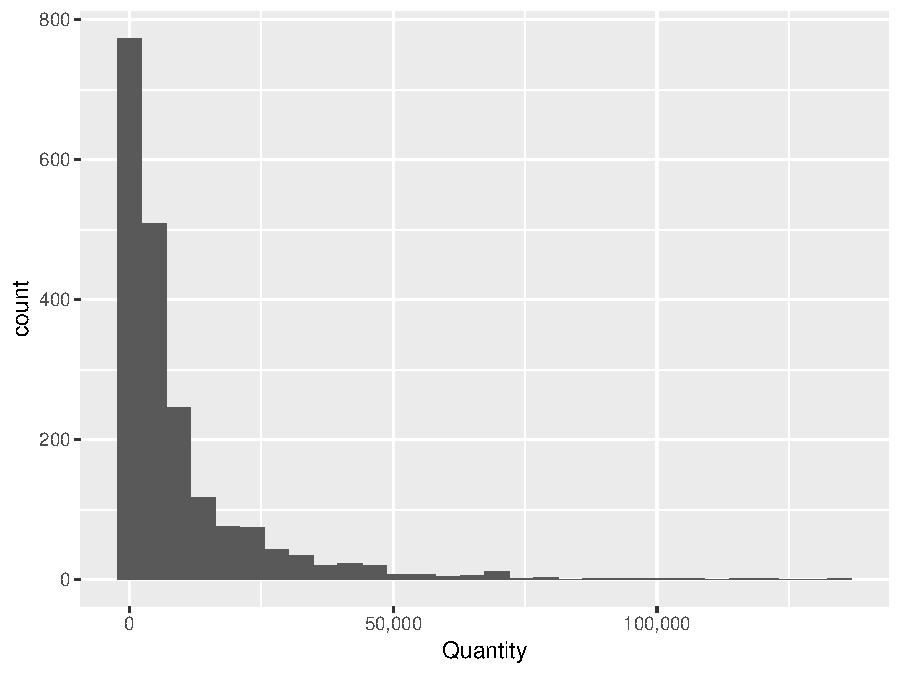
\includegraphics{UChicago-MScA-Capstone_files/figure-latex/Quantity-Histogram-1.pdf}
\caption{\label{fig:Quantity-Histogram}Histogram of Quantity}
\end{figure}
Quantity is not normally distributed but is instead heavily skewed left.
Large quantity orders are atypical and could have significant impact on
models.

\subsubsection{Distribution of Quantity over time \{methodology-QvsT
.unnumbered\}}\label{distribution-of-quantity-over-time-methodology-qvst-.unnumbered}

The figure below plots the aggregated Quantity over time.
\begin{figure}
\centering
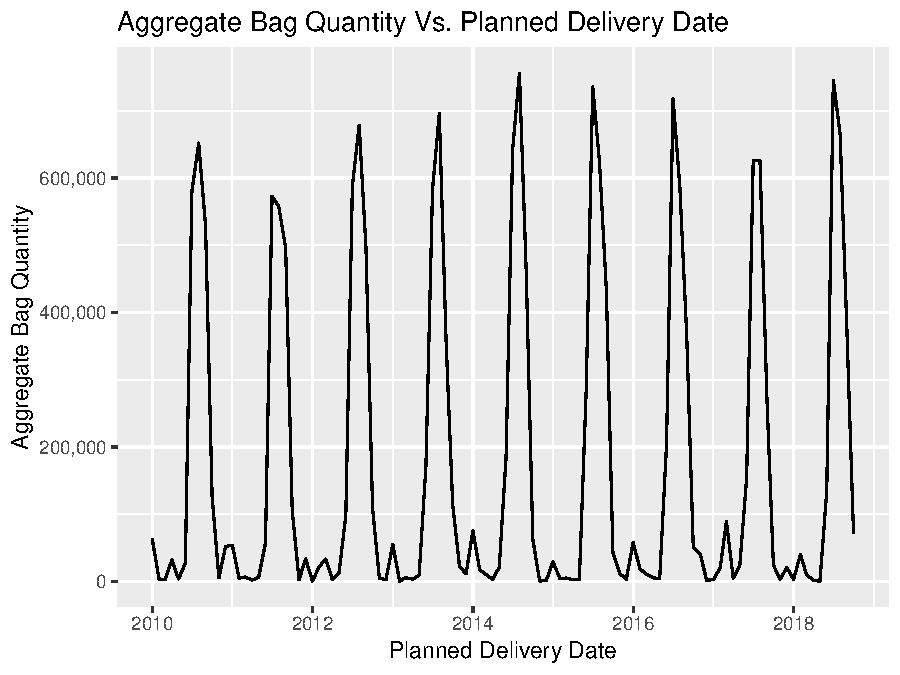
\includegraphics{UChicago-MScA-Capstone_files/figure-latex/Quantity-Time-1.pdf}
\caption{\label{fig:Quantity-Time}Quantity over Time}
\end{figure}
There is a large degree of seasonal behavior. Tomato bag shipments
increase during summer time from June to August and begin to drop off in
September and October. Quantity is very small during other months of the
year. This seasonality is easier to observe in the chart below which
aggregates bag shipments for each month of the year.
\begin{figure}
\centering
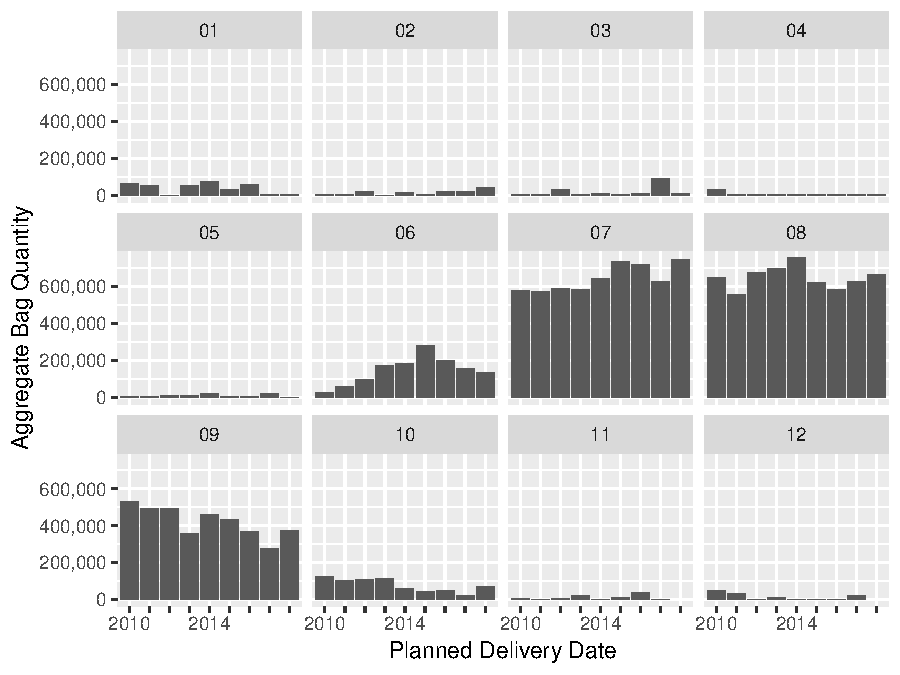
\includegraphics{UChicago-MScA-Capstone_files/figure-latex/Quantity-Month-1.pdf}
\caption{\label{fig:Quantity-Month}Monthy Quantity by Year}
\end{figure}
There is little year to year variation exhibited in each month, with the
possible exception of June which increased from 2010 to 2015 and then
decreased from 2016-2018.

\subsubsection*{Quantity by Item Number}\label{methodology-IN}
\addcontentsline{toc}{subsubsection}{Quantity by Item Number}

In addition to exploring the shipment quantity by time, we also observed
the effect that the Item Number on Quantity. Over 86\% of shipments are
driven by the top 10 out of a total of 60 item numbers.
\begin{figure}
\centering
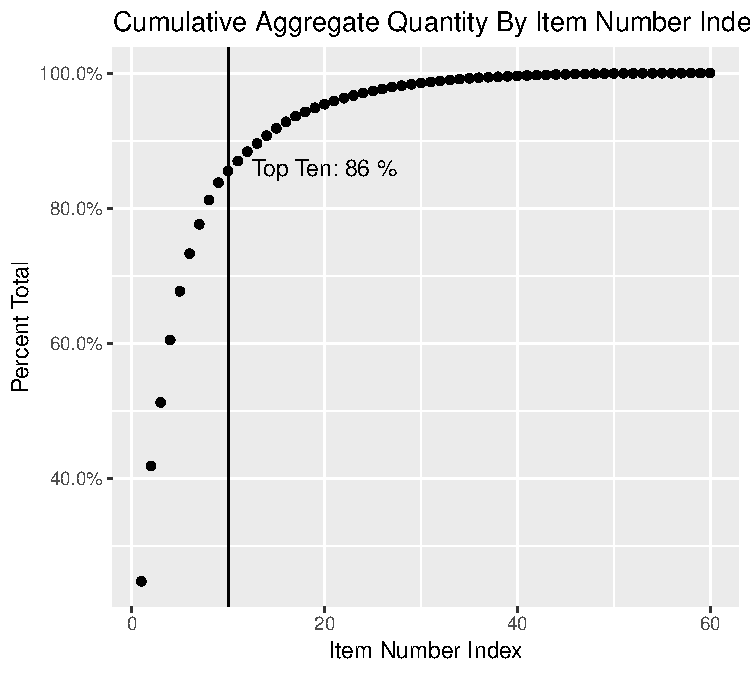
\includegraphics{UChicago-MScA-Capstone_files/figure-latex/IN-cumulative-1.pdf}
\caption{\label{fig:IN-cumulative}Cumulative Sales by Item Number}
\end{figure}
\begin{figure}
\centering
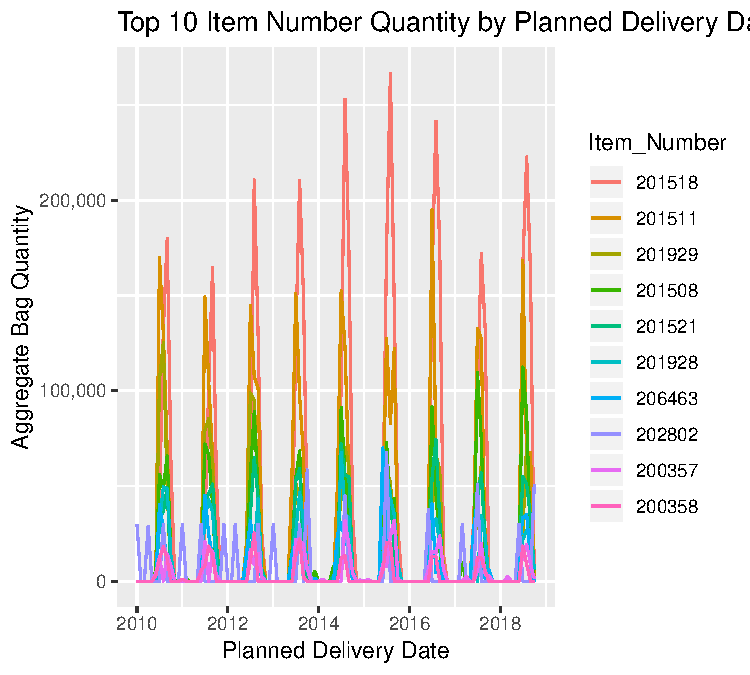
\includegraphics{UChicago-MScA-Capstone_files/figure-latex/IN-time-1.pdf}
\caption{\label{fig:IN-time}Top 10 Item Number Quantity over Time}
\end{figure}
Quantity by Item Number does not greatly vary greatly from the
aggregated Quantity. Because the seasonal nature of the data is so
strong, we will consider the shipment quantity aggregated to the monthly
level.

\section*{Descriptive analyses}\label{methodology-descriptive}
\addcontentsline{toc}{section}{Descriptive analyses}

\subsection*{External Data Collection}\label{methodology-external-data}
\addcontentsline{toc}{subsection}{External Data Collection}

Google engine search and twitter are important and representative social
media sources whose data is accessible. We collected social media data
from two sources: Twitter and the Google Trends. Google Trends
summarized US monthly search statistics from 2004 to 2019. The twitter
data collected are of US users from 2007 to 2018.

Google Trends returns a single value showing how frequently a given
search term (e.g. `Tomato') goes in Google's search engine relative to
its total search frequency for a given period.

Twitter data were gathered by collecting relevant tweets from Twitter
using key search words as shown in Table tab below. We can grab a tweet
based on defined keyword from Twitter by calling the Twitter API
function. Subsequently, we can categorize opinions expressed in a piece
of text, in order to determine opinion on our research (i.e, positive,
negative, or neutral).
\begin{longtable}[]{@{}rrrrr@{}}
\toprule
External Data Source & Frequency Granularity & Range & Size & Data
Type\tabularnewline
\midrule
\endhead
Google Trend & Monthly & 2004-2019 & 182 & Numeric\tabularnewline
Twitter & Monthly & 2007-2019 & & Text, Numeric\tabularnewline
\bottomrule
\end{longtable}
Table \ref{tab:External-Data} above shows the description of the social
media dataset. The google trend dataset based on relative search
frequency is on a monthly basis. The monthly dataset at the time of
reporting has 182 rows.

The Twitter data are sampled via a quasi-random approach that grabs data
monthly over the entire period of 2007 - 2018. We had to employ this
method of querying due to the nature of the Twitter API and its
restrictions on total tweets returned. The Twitter API returns tweets in
reverse chronological order. The total number of tweets that would
mention one of our keywords would be vastly larger than the number we
could collect over the course of our data collection period (January
2019 - March 2019). Limited in this way, we decided to strategically
collect tweets from each month of the year between January 2007 and
March 2019.

\textbf{Assumptions \& Limitations}

\textbf{Google Trends} Assumptions:
\begin{itemize}
\item
  We limited the Google Trends search to the United States.
\item
  The keywords are independent of each other.
\end{itemize}
Limitation:
\begin{itemize}
\tightlist
\item
  The actual number of searches for the term being queried is not made
  available. Instead, the data are reported from 0-100, where 100
  represents the maximum relative search frequency.
\end{itemize}
\textbf{Twitter Datasets} Assumptions:
\begin{itemize}
\item
  We limited Twitter data to the United States.
\item
  The frequency of tweets we collected for each keyword will be
  independent of the time period in which we collected them.
\end{itemize}
Limitations: * The demographic information of the twitter account user
cannot be determined.
\begin{itemize}
\item
  With the limitation of our premium account API activity, we can only
  submit 100 requests to collect tweet per month. Per each request, we
  can get a maximum of 500 tweets back.
\item
  The language associated with the Twitter account returned from the API
  does not guarantee the language of the Tweet. While we specified
  English language tweets, we received many tweets that were not in
  English. We subsequently dropped these tweets.
\end{itemize}
\textbf{Plan for use}

Working with Scholle, we developed a list of keywords to target in our
social media data collection. The keywords are listed in Table
\ref{tab:Keywords} below:
\begin{verbatim}
Warning in kable_markdown(x = structure(c("bbq", "chili", "ketchup",
"pasta", : The table should have a header (column names)
\end{verbatim}
\begin{longtable}[]{@{}cccccccc@{}}
\toprule
bbq & chili & ketchup & pasta & pizza & salsa & spaghetti &
tomato\tabularnewline
\bottomrule
\end{longtable}
Twitter data We developed a sentiment index for all tweets using natural
language processing techniques tilizing the textblob Library to analyze
how similar or discrepant the meaning of tweets among each keyword

Google Trends Correlation analysis of frequency of individual search
terms compared to quantity Subsequent seasonality \& trend analysis to
identify meaningful predictors

Twitter Data

We have collected tweets based on the keywords in Table below. Tweets
were aggregated on a monthly basis. The figure below shows how
frequently the keywords appears in the returned tweets over time. Pizza
is more frequently mentioned in Twitter than other keywords.

Google Trend Analysis

We collected Google Trend data consisting the same keywords as we did in
Tweet collection. The Google Trends data was standardized and
subsequently the cross correlation was found with respect to the Scholle
bag sales. Figure \ref{fig:ccf-google} displays the results of the cross
correlation analysis.
\begin{figure}

{\centering 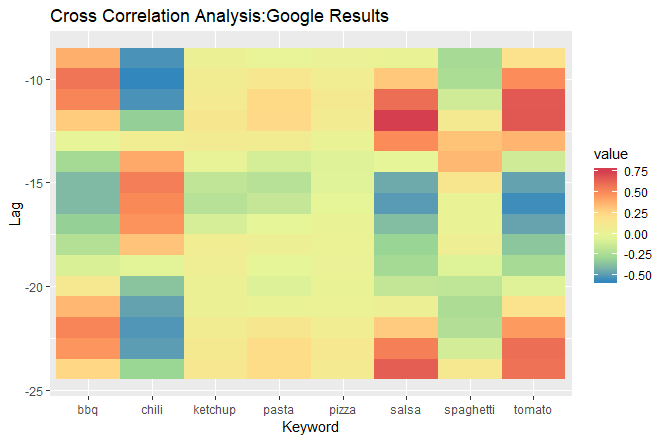
\includegraphics[width=400px]{figure/CCF_Google_Results} 

}

\caption{CCF Google}\label{fig:ccf-google}
\end{figure}
\begin{longtable}[]{@{}rrrrrrrr@{}}
\toprule
bbq & chili & ketchup & pasta & pizza & salsa & spaghetti &
tomato\tabularnewline
\midrule
\endhead
Lag 10 & Lag 15 & None & None & None & Lag 12 & None & Lag
12\tabularnewline
\bottomrule
\end{longtable}
In Table \ref{tab:Lags-Google} above, we highlight cross-correlations
greater than 0.5 and with a time period of greater than 8 months. Since
the Scholle bag sales data are records of the demand are placed well in
advance of the desired delivery date, we would expect a long lag window
in order for the trends of social media to drive market forces that
would affect demand. Red indicates positive relations and blue indicates
negative correlations. The deeper the color, the greater its correlation
with Scholle's data.

\subsection*{Tweet Sentiment Analysis}\label{tweet-sentiment-analysis}
\addcontentsline{toc}{subsection}{Tweet Sentiment Analysis}

We have conducted the following steps to conduct the sentiment analysis
of the tweets.

\textbf{Text Cleanup Pipeline:}
\begin{enumerate}
\def\labelenumi{\arabic{enumi}.}
\item
  Remove RT, URLs and non-text characters (except @ and punctuation
  symbols)
\item
  Handle mentions by replacing with upper case letters.
\item
  Remove all remaining non-text characters (including @ symbol and
  excluding punctuation symbols).
\item
  Check the language of the cleaned up tweet and drop any tweets that
  are not in English.
\end{enumerate}
\textbf{SpaCy Pipeline:}

We used the spaCy English Core Web Large model to analyze each tweet to
process into three data sets:
\begin{enumerate}
\def\labelenumi{\arabic{enumi}.}
\item
  Tokenization - each tweet was broken into its component elements of
  words, punctuation, etc.
\item
  Dependency Parsing - Annotate the tweet to add the syntactic
  dependency within the tweet i.e.~compare link verbs to their
  respective nouns.
\item
  Named Entities - Each tweet was analyzed to identify the named
  entities in the tweet. These entities will include the mentions
  because they were capitalized in the Text Cleanup Pipeline.
\item
  Removal of stop words - all stop words identified were removed.
\end{enumerate}
\textbf{Vector Extraction:}

Spacy includes vector representations for individual words as well as
entire entire sentences. See Figure below for the Keyword Distance using
Spacy.These are represented as 300 dimension Numpy arrays. To begin, we
confirmed that were was a reasonable cosine distance measure between
each of the keywords.
\begin{figure}

{\centering 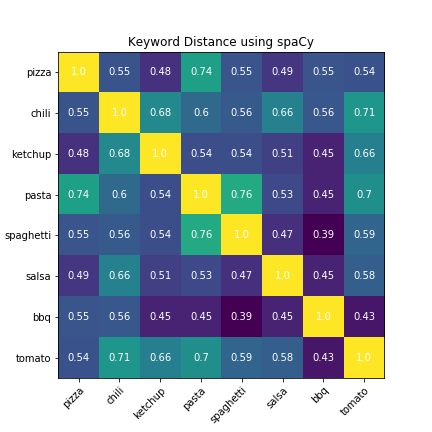
\includegraphics[width=400px]{figure/Keyword_Distance_Spacy} 

}

\caption{Spacy Keyword Vector Distance}\label{fig:spacy-keyword}
\end{figure}
There is a reasonable distance between each of the keywords with the
exception of bbq and barbecue but this is to be expected since they
reference the same thing.

In addition, vectors representations of each tweet can be extracted. For
each tweet keyword we summarised all vectors by finding their mean
values for each dimension. We then found the pairwise distance measures
for these `average' tweets. See in the figure below
\begin{figure}

{\centering 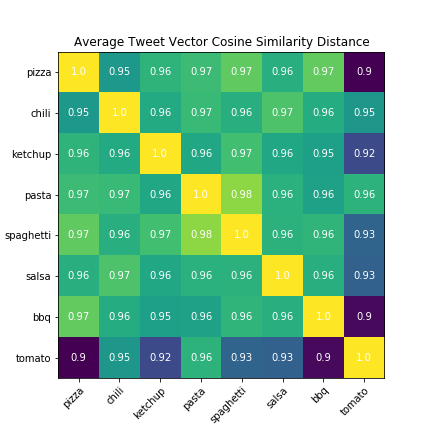
\includegraphics[width=400px]{figure/Tweet_Distance_Spacy} 

}

\caption{Spacy Average Tweet Vector Distance}\label{fig:spacy-average}
\end{figure}
Here, the ``average'' tweets are rather similar to each other with the
greatest distance from tomato to salsa.

In future work we will leverage these vector representations of the
tweets to conduct transfer learning to identify tweet sentiment.

\textbf{Sentiment Analysis using TextBlob}

TextBlob is an open source Python library for conducting natural
language processing. It has a built in sentiment analyzer that utilizes
two axes of analysis Polarity and Subjectivity. Polarity refers to a
positive or negative sentiment and ranges from positive one to negative
one respectively. Subjective expresses the subjectivity or objectivity
of the text. See Figure 24 below for the Tweet Polarity. The
subjectivity axis ranges from zero to positive one where 0 is very
objective and 1 is very subjective. See Figure 25 below for the Tweet
Subjectivity .
\begin{figure}

{\centering 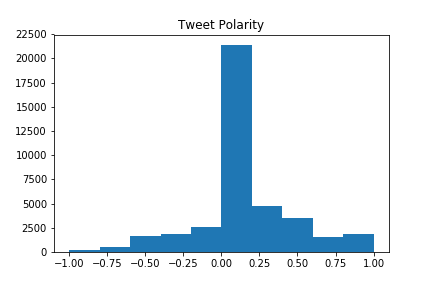
\includegraphics[width=400px]{figure/Tweet_Polarity} 

}

\caption{Textblob Tweet Polarity}\label{fig:tweet-polarity}
\end{figure}
\begin{figure}

{\centering 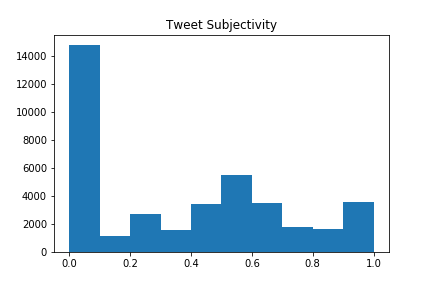
\includegraphics[width=400px]{figure/Tweet_Subjectivity} 

}

\caption{Textblob Tweet Subjectivity}\label{fig:tweet-subjectivity}
\end{figure}
\begin{figure}

{\centering 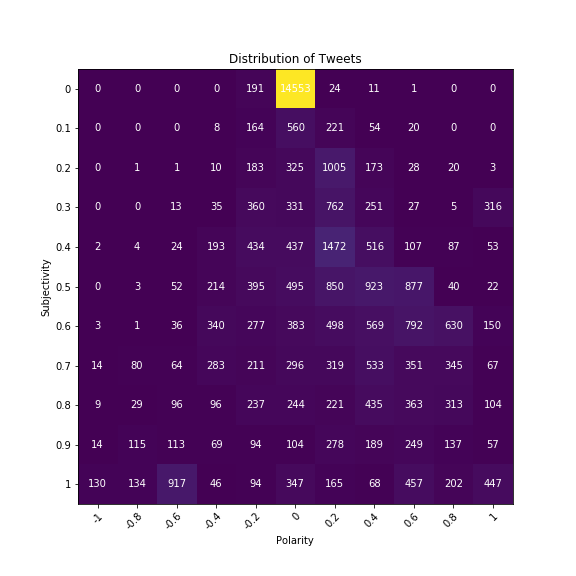
\includegraphics[width=400px]{figure/Tweet_Distribution} 

}

\caption{Textblob Tweet Distribution}\label{fig:tweet-distribution}
\end{figure}
TextBlob categorizes the vast majority of tweets as non-subjective
non-polar.

With the tweets collected, we generated a sentiment index by taking each
tweet's subjectivity \& polarity and multiplied them by the retweet
count for that tweet. We then aggregated the sentiment index at the
monthly level for each keyword. The cross correlation between the
Scholle data and the sentiment monthly index for the overall sentiment
and for each keyword was calculated and the results displayed in the
figure below.
\begin{figure}

{\centering 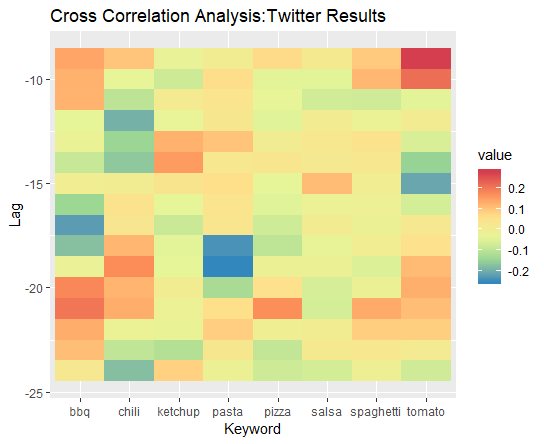
\includegraphics[width=400px]{figure/CCF_Twitter_Results} 

}

\caption{Twitter CCF Results}\label{fig:tweet-ccf}
\end{figure}
It is important to note the difference in scale relative to the Google
Trends results; the correlations to the Twitter sentiment index are much
weaker.

The table below compiles the list of lagged values used in our analysis.
\begin{longtable}[]{@{}rrrrrrrr@{}}
\toprule
bbq & chili & ketchup & pasta & pizza & salsa & spaghetti &
tomato\tabularnewline
\midrule
\endhead
Lag 17 & None & None & Lag 18 & None & None & None & Lag
15\tabularnewline
\bottomrule
\end{longtable}
\section*{Modeling Framework}\label{methodology-modeling}
\addcontentsline{toc}{section}{Modeling Framework}

\subsection*{Model Selection
Metrics}\label{methodology-ModelSelectionCriteria}
\addcontentsline{toc}{subsection}{Model Selection Metrics}

In order to determine the best model for predicting bag shipments, we
began by choosing selection metrics to test each model. The following
metrics outlined below will be used to measure the performance of each
model. 1. SMAPE 2. RMSE 3. \% bias -- no of time above forecast vs
below. 4. Accuracy

\textbf{sMAPE -Symmetric Mean Absolute Percentage Error}

Symmetric mean absolute percentage error (sMAPE) is an accuracy measure
based on percentage (or relative) errors. It allows us to understand
error independent of scale.

\[sMAPE=\frac{100\%}{n}\frac{|A_t-F_t|}{(|A_t|+|F_t|)/2}\]

sMAPE has a lower bound of 0\% and an upper bound of 100\%. The best
value is 0\% while the worst value is 100\%.

The major limitation with sMAPE is that it gives more penalties to
underestimates than overestimates.

\textbf{RMSE - Root Mean Squared Error}

The root mean squared error (RMSE) of an estimator measures the average
of the squares of the errors---that is, the average squared difference
between the estimated values and what is estimated. The square root of
this value is then taken to produce the RMSE.

\[RMSE = \sqrt{\frac{\sum^n(A_t-F_t)^2}{n}}\]

RMSE measures the variation between predicted and measured values and it
provides us a basis for measuring the model variance on the same scale
as the data.

The RMSE is a measure of the quality of an estimator. RMSE is always
non-negative, as the process of squaring removes any negative signs. It
also penalizes larger differences. The best value is zero while the
worst value is unbounded.

In sum, the lower the RMSE, the smaller the error, the better the
estimator.

\textbf{Percent Bias -- ratio of model high or low.}

Bias refers to the propensity of a measurement process to over- or
under-estimate the value of a population parameter. Percent bias (PBIAS)
measures the average tendency of the predicted values to be larger or
smaller than the actual values.

Percent Bias is calculated by taking the sign of the residual for each
data point and setting positive values to 1 and negatives values to
zero. These are then averaged and multiplied by 100 to produce a
percentage. The best percentage bias is 50\% - there are just as many
over predictions as under predictions. The worst percentage bias is
either 0\% or 100\% as the model is regularly over- or under-estimating
the actual data.

\textbf{Accuracy - Mean Accuracy between Model \& Actual}

Accuracy measures the closeness of a model prediction to the actual
value. In our case we are measuring the mean accuracy for all model
predictions versus actual values. The best accuracy measure is 1; the
prediction and the actual are the same so their ratio is 1. Accuracies
that diverge from 1 are bad; a value greater than 1 means the prediction
was higher than the actual while a value below 1 is means the
predictions was lower than the actual. We aggregate the accuracy measure
for each data point and find the overall mean. One precaution to
consider by using this procedure is it may mask an underlying trend in
prediction of the accuracy in which the model could overestimate early
and then underestimate late or other non-linear behavior.

\subsection*{Additional Modeling
Considerations}\label{methodology-AdditionalConsiderations}
\addcontentsline{toc}{subsection}{Additional Modeling Considerations}

\textbf{Training and Forecasting Windows}

In order to evaluate our model to avoid either overfitting or
underfitting , we split our dataset into a training set and a test set.
Based on our discussions with Scholle, the test set will be the
subsequent 18 months. The length of the training period was chosen based
on the evaluation of the model stability of our baseline model using a
rolling window cross validation.

\textbf{Rolling Window Cross Validation}

Time series data present a unique challenge in analysis in that the data
are not independent - they are collected at regular intervals over the
course of time. We employed rolling window cross validation to generate
multiple train and test sets from the overall data set. Initially we
explored the model stability of our baseline model and used the best
criteria from that in order to decide the length of the cross validation
window.

\chapter*{Findings}\label{findings}
\addcontentsline{toc}{chapter}{Findings}

\section*{Results of descriptive analyses}\label{findings-descriptive}
\addcontentsline{toc}{section}{Results of descriptive analyses}

Because of the highly seasonal nature of the data, we created a baseline
model using only Scholle data. We used periods of 2-year, 4-year and
6-year windows, to identify the forecast window period with the greatest
stability.

\subsection*{Baseline Model - Prophet}\label{findings-baseline}
\addcontentsline{toc}{subsection}{Baseline Model - Prophet}

Prophet is an open-source tool developed by Facebook to conduct time
series modeling. Prophet models data using a decomposable time series
model with three main components: trend, seasonality, and holidays. The
focus is to model the time series via regression instead of as a
generative model like ARIMA would. This is done for flexibility, the
ability to handle irregularly spaced data, speed, and interpretability.

\textbf{Cross-Validation Window Selection}

The figures below show results of the cross-validation analysis at 2, 4
and 6 year training windows using the Prophet Model.
\begin{figure}

{\centering 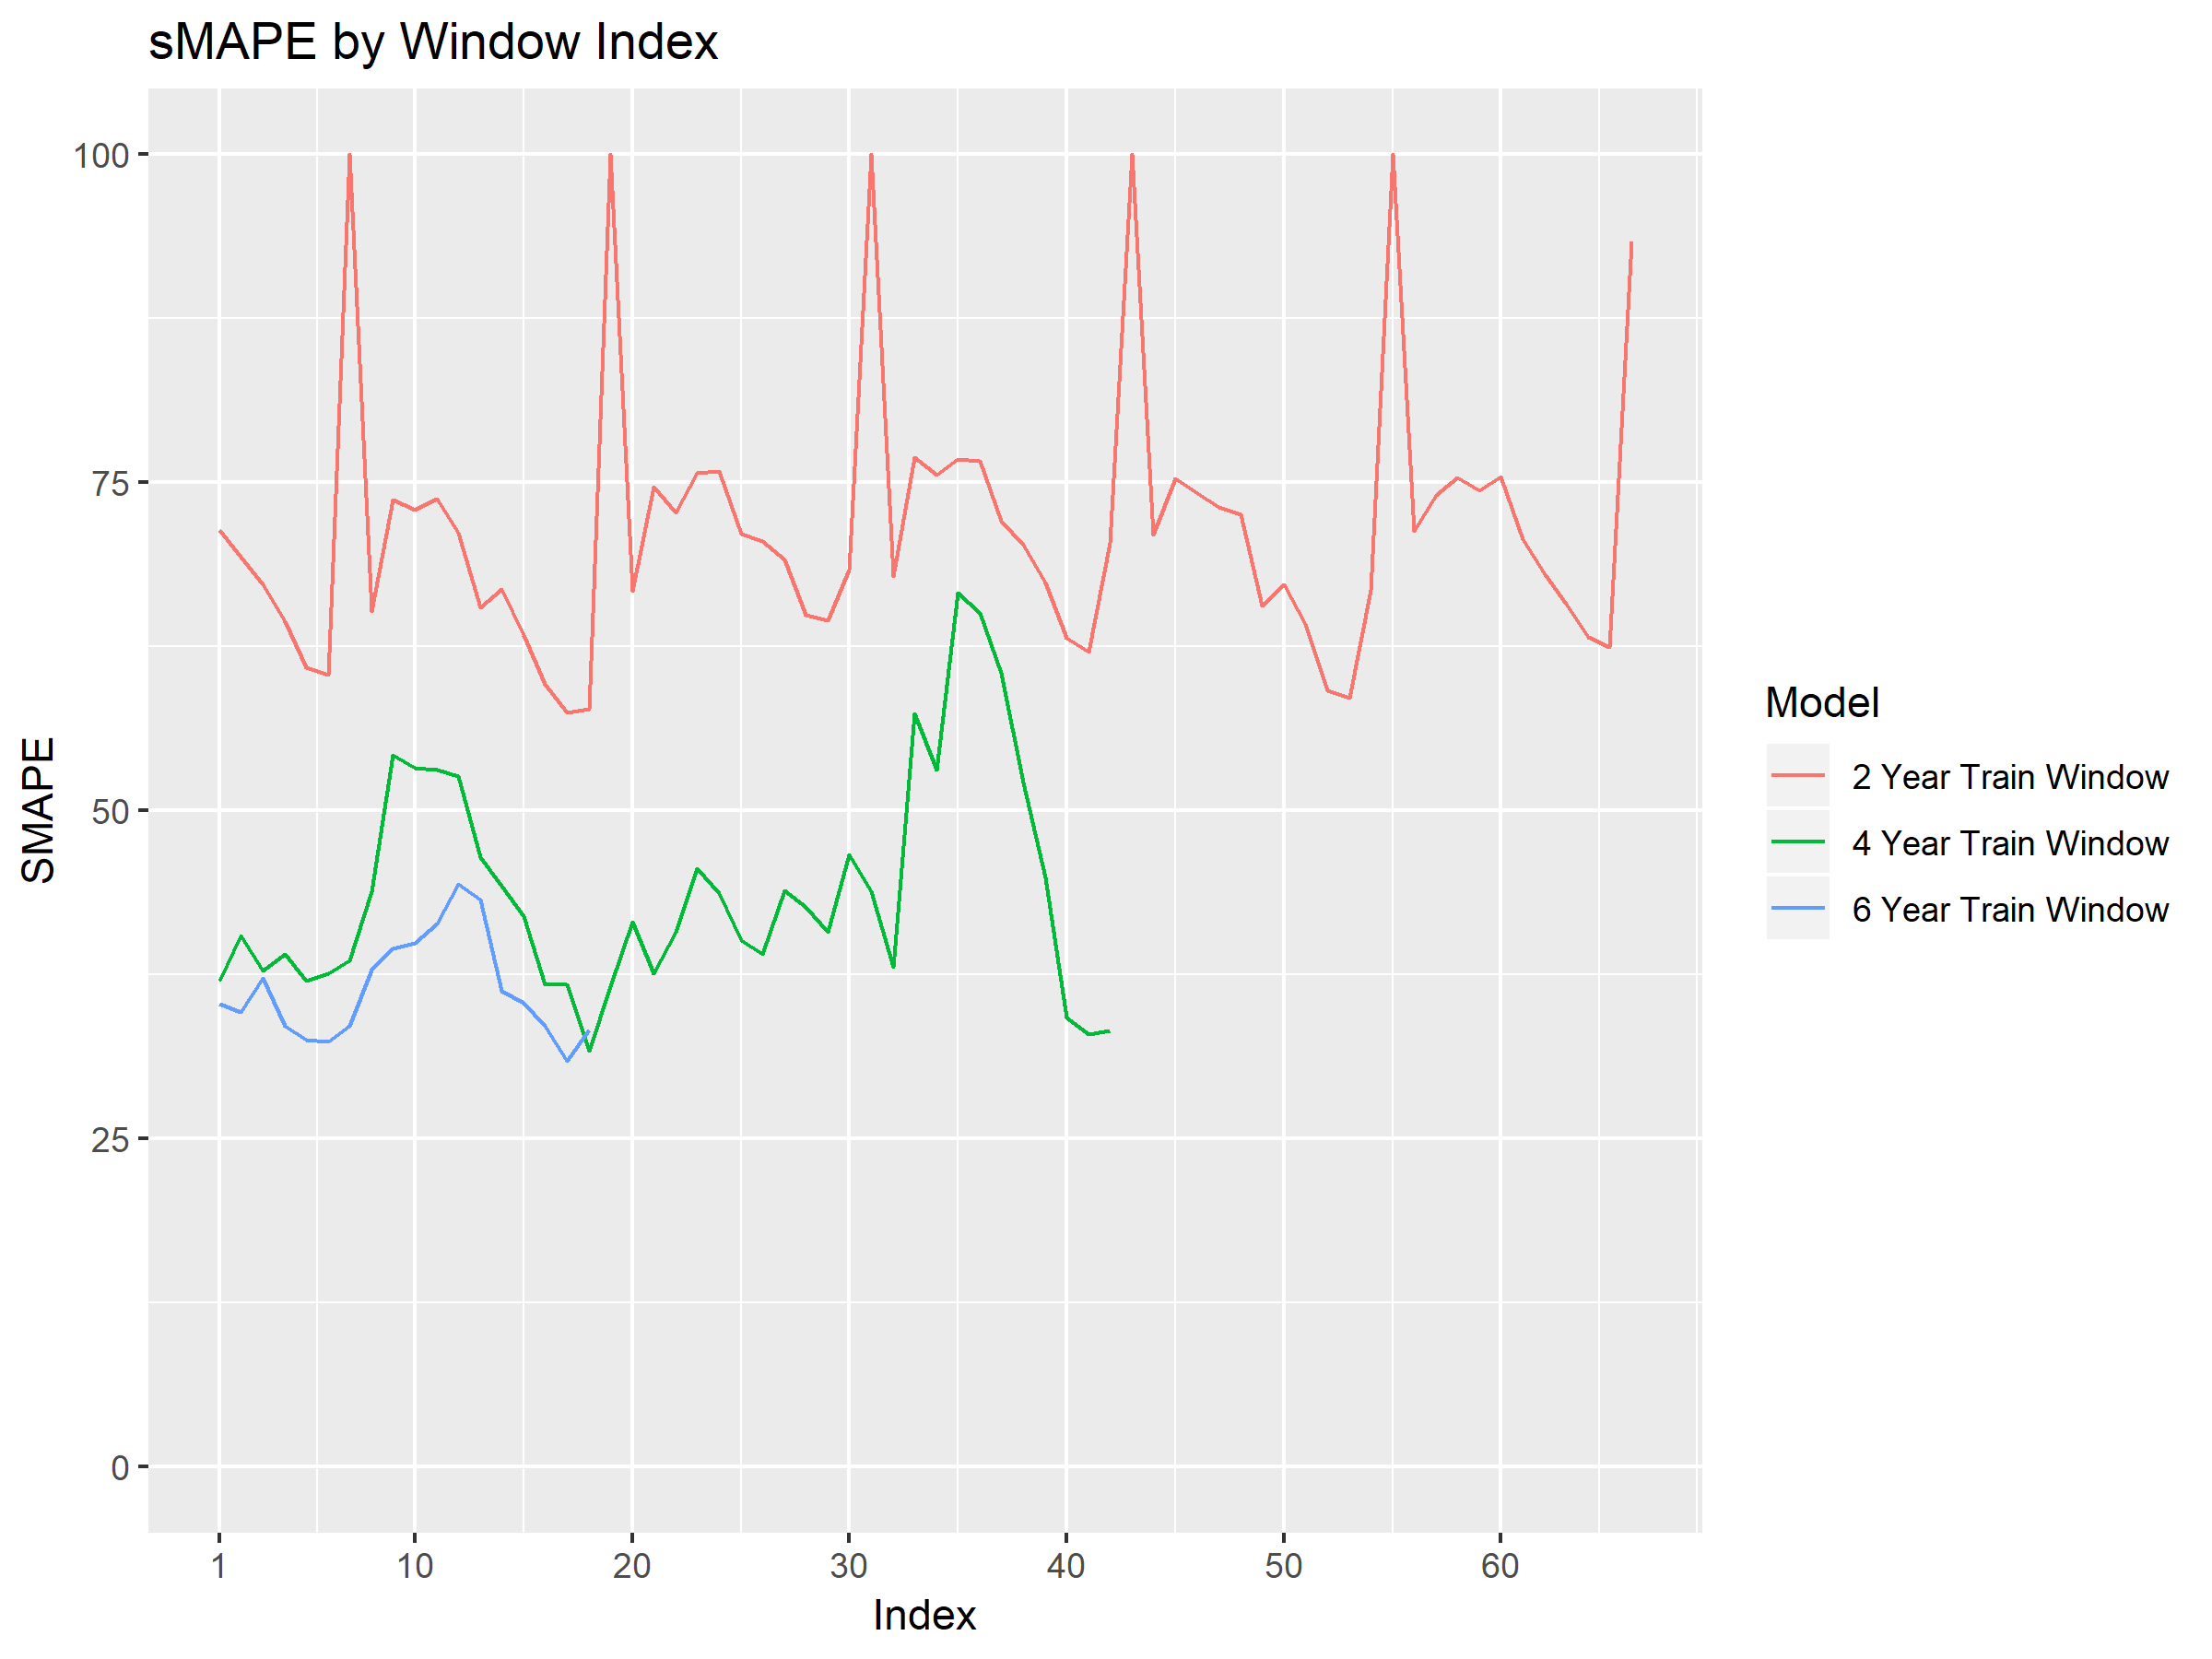
\includegraphics[width=400px]{figure/Prophet_SMAPE_CV} 

}

\caption{2 4 and 6 year cross validation of Prophet models - sMAPE}\label{fig:cross-val-selection-smape}
\end{figure}
\begin{figure}

{\centering 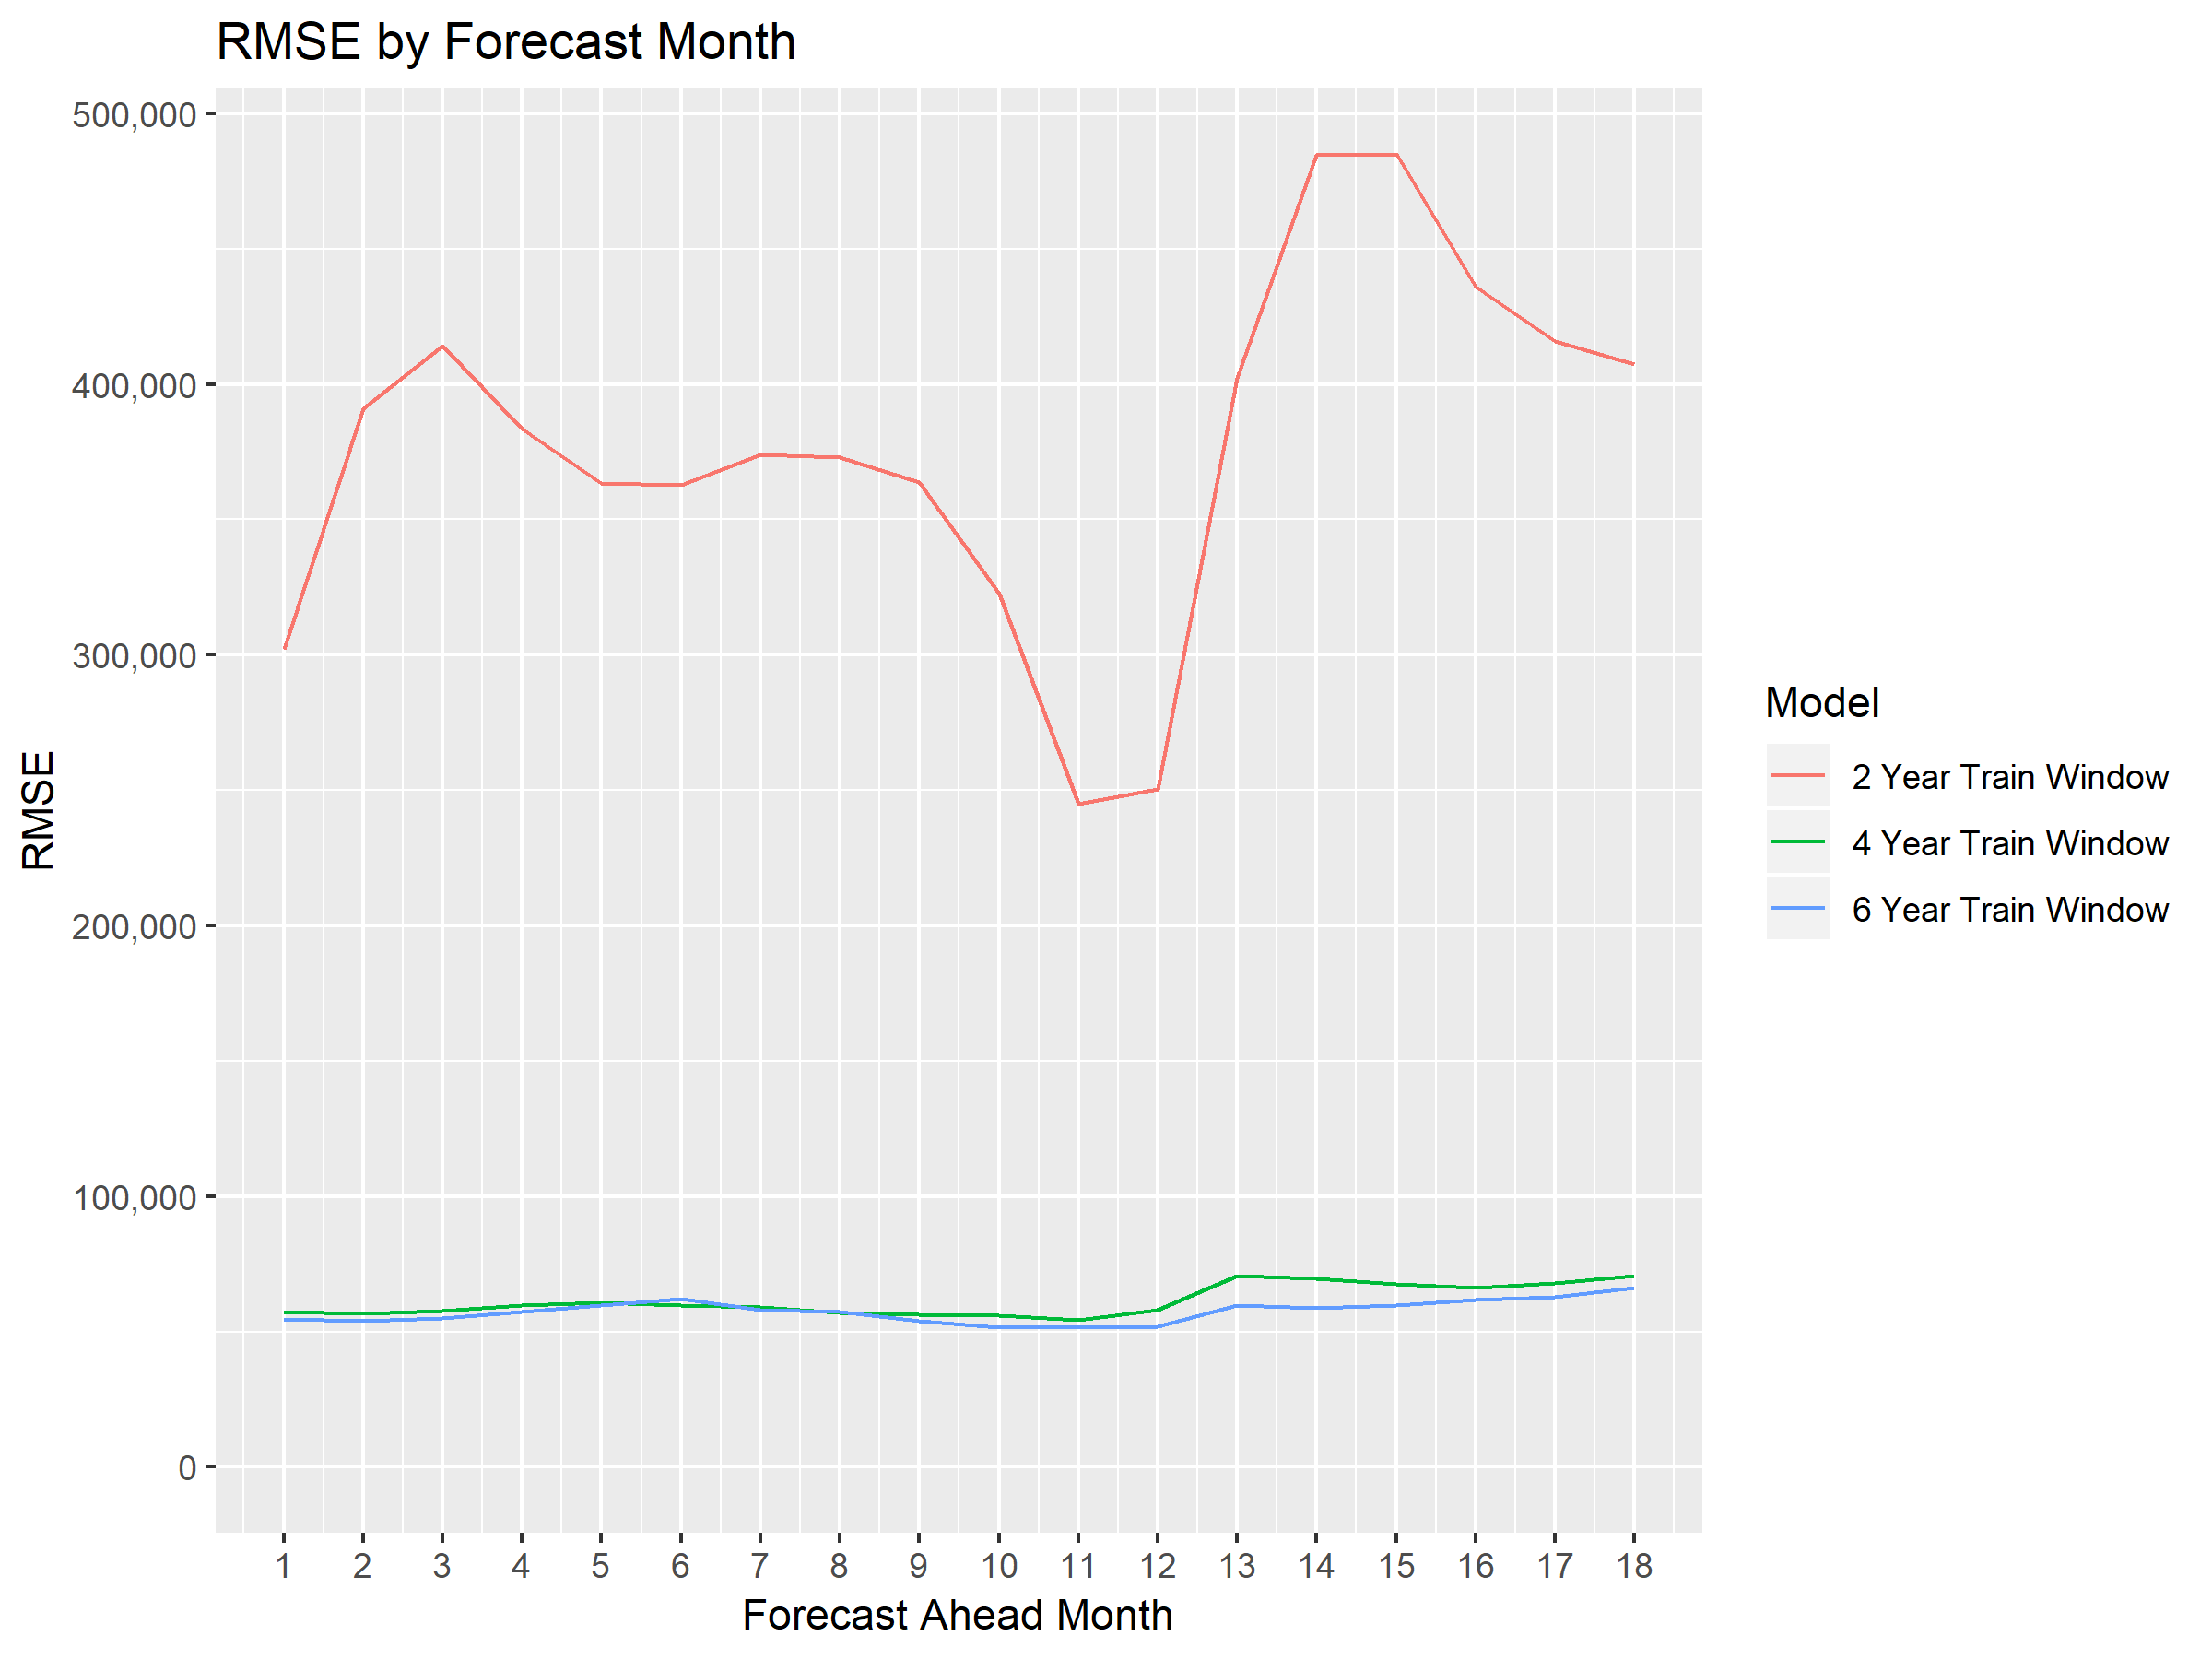
\includegraphics[width=400px]{figure/Prophet_RMSE_CV} 

}

\caption{2 4 and 6 year cross validation of Prophet models - RMSE}\label{fig:cross-val-selection-rmse}
\end{figure}
For both sMAPE and RMSE, the 2 year window shows much higher variability
than the 4 or 6 year windows. Given the similarity of the 4 and 6 year
windows RMSE, we chose the 4 year window to both reduce the data
requirements of the model and allow for additional cross-validation of
each other model. A 4 year cross validation allows us to generate 42
complete training and testing windows whereas A 6 year cross validation
window only allows us to generate 18.

\textbf{Baseline Model Results}

The reported model metrics are the mean values for each of the cross
validation periods collected.
\begin{longtable}[]{@{}rrrrr@{}}
\toprule
X & sMAPE & RMSE & X..Bias & Accuracy\tabularnewline
\midrule
\endhead
Train & 30\% & 29896.68 & 22\% & 0.86\tabularnewline
Test & 43\% & 62625.69 & 67\% & 4.04\tabularnewline
\bottomrule
\end{longtable}
\subsection*{Challenger Model sARIMA}\label{findings-sARIMA}
\addcontentsline{toc}{subsection}{Challenger Model sARIMA}

Seasonality is a key feature of the dataset, as it was observed that the
Tomato bags sales increase significantly during summer time from June to
August and drop in September and October while repeating this cycle
annually.This key attribute in the dataset meant we deploy a model that
uses differencing at a lag equalling the number of seasons to remove
additive seasonal effect.

For this challenger, we split the data into two groupings; harvest
months (June -October) and all months. In the Table 7 \& 8 below, we
summarise the result for the model:
\begin{longtable}[]{@{}rrrrr@{}}
\toprule
X & sMAPE & RMSE & X..Bias & Accuracy\tabularnewline
\midrule
\endhead
Train & 9\% & 125522.0 & 19\% & 1.76\tabularnewline
Test & 68\% & 338725.3 & 100\% & 0.43\tabularnewline
\bottomrule
\end{longtable}
In the figure below, the mean forecast value is highlighted in blue and
the actual value is captured in red, and the confidence interval ranging
between 80\%-95\%. The actual values are represented in black.
\begin{figure}

{\centering \includegraphics[width=400px]{figure/Arima_12month} 

}

\caption{12 Month Arima}\label{fig:arima-12}
\end{figure}
\begin{figure}

{\centering 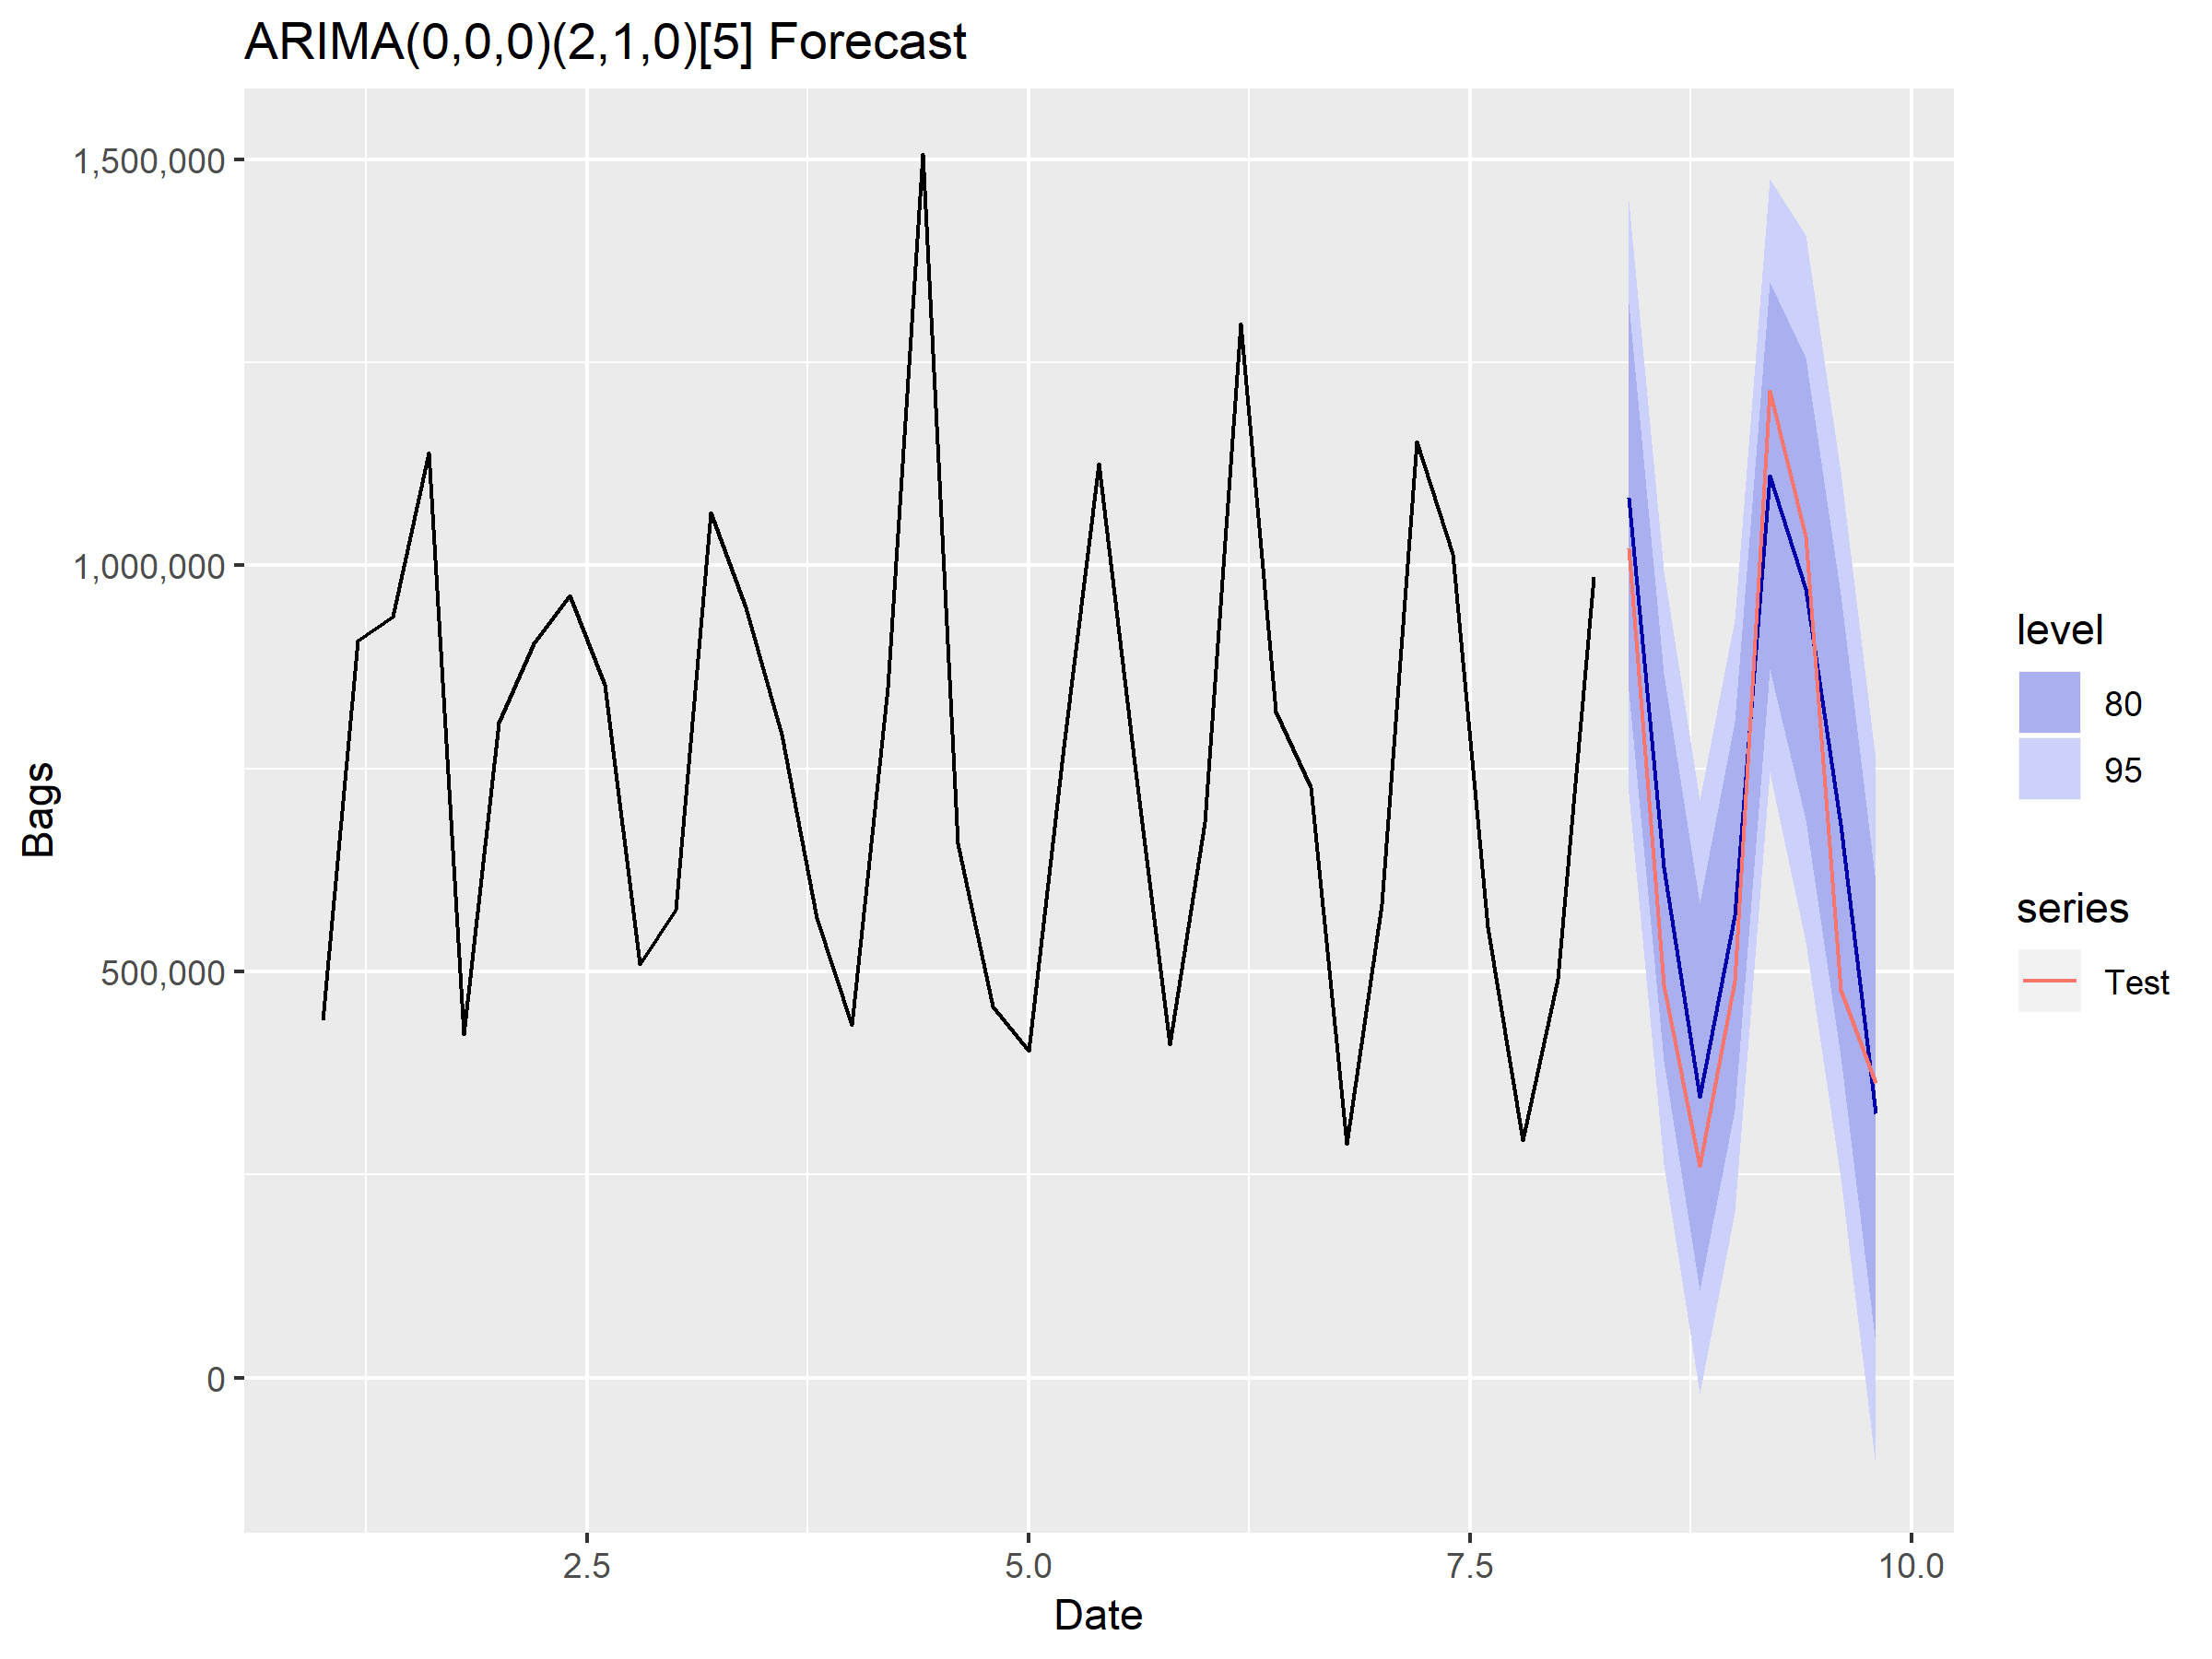
\includegraphics[width=400px]{figure/HarvestArima} 

}

\caption{Harvest (June-October) Month Arima}\label{fig:arima-5}
\end{figure}
The Arima model, especially for the harvest months, provides a
compelling challenge due to its simplicity.

\subsection*{Challenger Model - Regression with ARIMA
Errors}\label{findings-Regression}
\addcontentsline{toc}{subsection}{Challenger Model - Regression with
ARIMA Errors}

The next challenger model we built is a linear regression model with
ARIMA errors. While the regression model allows for the inclusion of
predictor variables, it does not allow for the subtle time series
dynamics that can be handled by ARIMA models. The regression with ARIMA
errors model solves this problem by fitting regression models with all
the relevant variables first, and then applying ARIMA to the residuals
of the regression to detect time series elements in the residuals.

We explored the correlations of twitter data and Google trend Scholle
tomato bag sales and found the keywords and lags in Table 4 and Table 6
tend to strongly correlated with tomato bag sales. Since the regression
with ARIMA errors is based on linear regression, we first build a linear
regression model these keywords and lags. Results are shown in below
Table \_ . Significant variables are highlighted in green.

Based on the variables significant in the linear model, we built the
regression model with ARIMA errors. The parameters and accuracy are
shown below in Table and Table .
\begin{longtable}[]{@{}rrr@{}}
\toprule
Keyword\ldots{}Lag & Estimate & P.Value\tabularnewline
\midrule
\endhead
Intercept & 114883 & 0.00\tabularnewline
bbq\_twitter\_lag17 & -7771 & 0.48\tabularnewline
pasta\_twitter\_lag18 & 7946 & 0.74\tabularnewline
tomato\_twitter\_lag15 & 2645 & 0.80\tabularnewline
Google bbq lag 10 & -39516 & 0.14\tabularnewline
Google chili lag 15 & -42963 & 0.02\tabularnewline
Google salsa lag 12 & 92606 & 0.00\tabularnewline
Google tomato lag 12 & 122522 & 0.00\tabularnewline
\bottomrule
\end{longtable}
Based on the variables significant in the linear model, we built the
regression model with ARIMA errors. The parameters and accuracy are
shown below in Table and Table .
\begin{longtable}[]{@{}rrr@{}}
\toprule
Keyword\ldots{}Lag & Estimate & P.Value\tabularnewline
\midrule
\endhead
Google bbq lag 10 & -39516 & 0.137173\tabularnewline
Google chili lag 15 & -42963 & 0.017008\tabularnewline
Google salsa lag 12 & 92606 & 0.000366\tabularnewline
Google tomato lag 12 & 122522 & 0.000145\tabularnewline
\bottomrule
\end{longtable}
Positive coefficients imply that for a unit increase in the variable,
there is a corresponding positive increase in the Scholle bag sales.
Negative coefficients imply that for a unit increase in the variable,
there is a corresponding negative decrease in the Scholle bag sales.The
negative coefficient shows there is an inverse relationship between the
variable and Scholle bag sales.
\begin{longtable}[]{@{}rrrrr@{}}
\toprule
X & sMAPE & RMSE & X..Bias & Accuracy\tabularnewline
\midrule
\endhead
Train & 25\% & 93857.76 & 20\% & 0.38\tabularnewline
Test & 44\% & 68342.19 & 58\% & -0.93\tabularnewline
\bottomrule
\end{longtable}
The above results indicate that Google trend data tend to have a greater
influence in the predictions than twitter data, because the count in
google searches is more direct in measuring the importance of the
keywords and lags, compared to twitter data which might lose some
information both due to the limitations in gathering tweet data and due
to the complicated natural language preprocessing process. The ARIMA
error is (1,0,0),(0,1,2){[}12{]}, indicating that the regression data
was not sufficient to capture the time series elements of the data.

\subsection*{Challenger Model - Random Forest
Regression}\label{findings-RF}
\addcontentsline{toc}{subsection}{Challenger Model - Random Forest
Regression}

The second challenger model we built was a Random Forest Regression
Model. Random Forest leverages many regression trees to build a
consensus model in addition to bootstrap aggregation or bagging to
generate additional augmented data. Bagging simply builds additional
training sets by sampling with replacement from provided training data.
Each individual tree uses the bagged training data and selects a random
subset of features at each branching point rather than all features
available to build the regression. This restriction forces the model to
create a more robust estimator.

One useful feature when using tree-based approaches for regression is
the ability to use categorical or ordinal predictors without the need
for one-hot-encoding. In our model we represented the date as a pair of
categorical variables, one for year and a second for month. We chose to
do this because of the seasonal nature of the data.

In addition, we decided to challenge the model by only using lags that
we thought to be have a reasonable explanation for their effect. To this
end we chose to use lags greater than 9 months. Our logic was that it
would take time for an increase or decrease in the social media presence
of one of the keywords selected to go from an uptick in interest of
consumer products to be captured by Scholle's bag sales.

The table below displays the results of our Random Forest model.
\begin{longtable}[]{@{}rrrrr@{}}
\toprule
X & sMAPE & RMSE & X..Bias & Accuracy\tabularnewline
\midrule
\endhead
Train & 38\% & 66560.6 & 64\% & 2.94\tabularnewline
Test & 37\% & 61758.7 & 28\% & 5.54\tabularnewline
\bottomrule
\end{longtable}
An important feature of Random Forest modelling is its ability to
generate rank-ordered summaries of variable importance. The model's
feature importance is displayed in the figure below.
\begin{figure}
\centering
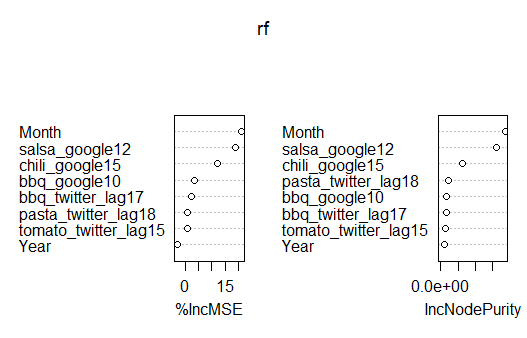
\includegraphics{./figure/RF_V_Imp.png}
\caption{Random Forest Importance}
\end{figure}
The most important features are displayed at the top of this chart, in
this the month was the most important predictor followed closely by
google salsa data at lag 12. This agrees with the importance of monthly
seasonality that we observed in the other models.

\subsection*{Challenger Model - XGBoost}\label{findings-XGBoost}
\addcontentsline{toc}{subsection}{Challenger Model - XGBoost}

XGBoost is an implementation of gradient boosted decision trees designed
for speed and performance. It build trees one at a time, where each new
tree helps to correct errors made by previously trained tree.
\begin{longtable}[]{@{}rrrrr@{}}
\toprule
X & sMAPE & RMSE & X..Bias & Accuracy\tabularnewline
\midrule
\endhead
Train & 15\% & 55311.64 & 11\% & 0.52\tabularnewline
Test & 35\% & 88097.99 & 44\% & 2.00\tabularnewline
\bottomrule
\end{longtable}
\subsection*{Stacking Forecasts}\label{findings-Stacking}
\addcontentsline{toc}{subsection}{Stacking Forecasts}

Our project focuses on shipment quantity. There will inherently be some
lag between the time someone has interaction on social media and its
effect on the tomato bag shipments. Given that the vast majority of
shipments occur during June through October, we limited the evaluation
of model results to those months. These months coincide with when
tomatoes become ripe in California, we thus refer to these months as the
harvest months.

The stacking method is used to create an additional consensus model by
using the results of trained models. We used two approaches to stacking,
simple averaging and a linear model.

We then combined our forecast results from all models mentioned prior in
this report, including the ARIMA model built only on the more stationary
harvest months, the regression with ARIMA errors model using on strong
correlated keywords and lags, random forest model, XGBoost model and
Prophet model. We averaged the forecasts of all combinations of the
models. We found that we were able to improve the model predictions by
combining the Random Forest and Regression with Arima Error models
predictions using a simple average.

The second approach to stacking we attempted was to build a linear model
using the results of all our other models. This model was trained on all
the harvest month data for 2014-2018. An important facet of a linear
model is that it optimizes the weighting of each variable. Our case this
is the model result. The fitted values produced a better estimate of the
actual than the simple average of Random Forest and Regression with
Arima Error.
\begin{longtable}[]{@{}lr@{}}
\toprule
& x\tabularnewline
\midrule
\endhead
Intercept & -6428.4630100\tabularnewline
Arima & 0.7431722\tabularnewline
Arima\_reg & -0.1683120\tabularnewline
RF & 0.6933001\tabularnewline
xgb & 0.3950322\tabularnewline
pro & -0.5076684\tabularnewline
\bottomrule
\end{longtable}
However the best fitting linear model does not consider if each of the
inputs adds to the total information that is represented in each of the
variables added. To address this, we applied the step function to find
the model that produces the lowest AIC.

Overall the linear model blend performed the best for both sMAPE and
RMSE leading us to choose it as our champion model.

key: * arima - * arima\_reg - * xgb - * pro -
\begin{longtable}[]{@{}rrrrr@{}}
\toprule
Model & sMAPE & RMSE & X..Bias & Accuracy\tabularnewline
\midrule
\endhead
arima & 12.76369 & 369493.5 & 0.48 & 1.0930270\tabularnewline
arima\_reg & 11.59555 & 378343.2 & 0.52 & 1.1734880\tabularnewline
RF & 12.75160 & 427591.7 & 0.36 & 1.0892416\tabularnewline
xgb & 19.91717 & 611248.7 & 0.32 & 0.9974092\tabularnewline
pro & 16.30583 & 393135.5 & 0.56 & 1.1628570\tabularnewline
tot\_avg & 12.82756 & 362912.5 & 0.44 & 1.1032046\tabularnewline
arima+arima\_reg & 11.99662 & 366844.9 & 0.52 & 1.1332575\tabularnewline
arima+RF & 11.06201 & 339078.2 & 0.44 & 1.0911343\tabularnewline
arima+xgb & 14.08614 & 412555.8 & 0.36 & 1.0452181\tabularnewline
arima+pro & 13.66767 & 345109.6 & 0.48 & 1.1279420\tabularnewline
arima\_reg+RF & 11.02261 & 345499.1 & 0.48 & 1.1313648\tabularnewline
arima\_reg+xgb & 13.47914 & 417879.0 & 0.36 & 1.0854486\tabularnewline
arima\_reg+pro & 12.96459 & 348679.2 & 0.56 & 1.1681725\tabularnewline
RF+xgb & 15.06955 & 494505.8 & 0.36 & 1.0433254\tabularnewline
RF+pro & 13.95099 & 378280.1 & 0.52 & 1.1260493\tabularnewline
xgb+pro & 17.60323 & 473411.7 & 0.48 & 1.0801331\tabularnewline
arima+arima\_reg+RF & 11.33500 & 335521.4 & 0.52 &
1.1185856\tabularnewline
arima+arima\_reg+xgb & 12.76800 & 374804.7 & 0.52 &
1.0879748\tabularnewline
arima+arima\_reg+pro & 12.82931 & 344284.7 & 0.52 &
1.1431240\tabularnewline
arima\_reg+RF+xgb & 12.61945 & 402010.3 & 0.40 &
1.0867130\tabularnewline
arima\_reg+RF+pro & 12.19553 & 342480.6 & 0.52 &
1.1418622\tabularnewline
RF+xgb+pro & 12.61945 & 402010.3 & 0.40 & 1.0867130\tabularnewline
Linear Model Blend & 10.95078 & 297958.3 & 0.56 &
1.1296389\tabularnewline
\bottomrule
\end{longtable}
\subsection*{Residual Analysis}\label{findings-Residual-Analysis}
\addcontentsline{toc}{subsection}{Residual Analysis}
\begin{Shaded}
\begin{Highlighting}[]
\CommentTok{#plot each of the forecasts & the blend & actual}
\end{Highlighting}
\end{Shaded}
Residual analysis is an important final step because it helps us
understand if our model has any systemic biases that we should be aware
of going forward.
\begin{Shaded}
\begin{Highlighting}[]
\NormalTok{lm_blender <-}\StringTok{ }\KeywordTok{readRDS}\NormalTok{(}\StringTok{'./data/LM_Blender.rds'}\NormalTok{)}
\KeywordTok{par}\NormalTok{(}\DataTypeTok{mfrow=}\KeywordTok{c}\NormalTok{(}\DecValTok{2}\NormalTok{,}\DecValTok{2}\NormalTok{))}
\KeywordTok{plot}\NormalTok{(lm_blender)}
\end{Highlighting}
\end{Shaded}
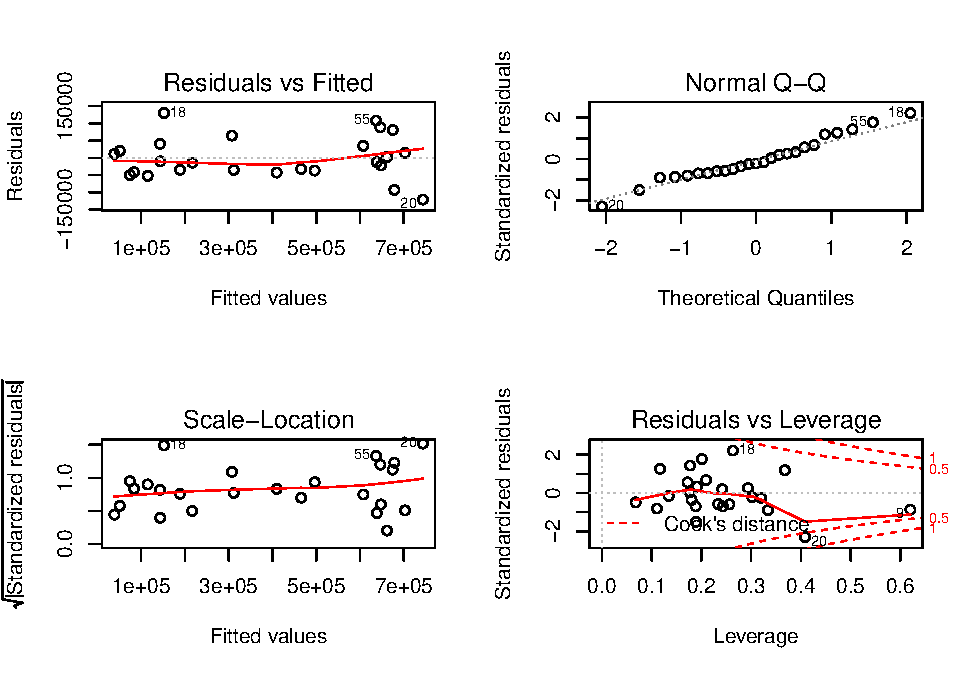
\includegraphics{UChicago-MScA-Capstone_files/figure-latex/unnamed-chunk-3-1.pdf}
\begin{Shaded}
\begin{Highlighting}[]
\KeywordTok{par}\NormalTok{(}\DataTypeTok{mfrow=}\KeywordTok{c}\NormalTok{(}\DecValTok{1}\NormalTok{,}\DecValTok{1}\NormalTok{))}
\end{Highlighting}
\end{Shaded}
\begin{Shaded}
\begin{Highlighting}[]
\NormalTok{facts =}\StringTok{ }\KeywordTok{c}\NormalTok{(}\DataTypeTok{mean =} \KeywordTok{mean}\NormalTok{(lm_blender}\OperatorTok{$}\NormalTok{residuals),}
          \DataTypeTok{median =} \KeywordTok{median}\NormalTok{(lm_blender}\OperatorTok{$}\NormalTok{residuals),}
          \DataTypeTok{variance =} \KeywordTok{var}\NormalTok{(lm_blender}\OperatorTok{$}\NormalTok{residuals),}
          \DataTypeTok{skewness =}\NormalTok{ e1071}\OperatorTok{::}\KeywordTok{skewness}\NormalTok{(lm_blender}\OperatorTok{$}\NormalTok{residuals),}
          \DataTypeTok{kurtosis =}\NormalTok{ e1071}\OperatorTok{::}\KeywordTok{kurtosis}\NormalTok{(lm_blender}\OperatorTok{$}\NormalTok{residuals))}
          
\NormalTok{kableExtra}\OperatorTok{::}\KeywordTok{kable}\NormalTok{(facts, }\DataTypeTok{digit =} \DecValTok{2}\NormalTok{, }\DataTypeTok{align =} \StringTok{"r"}\NormalTok{, }\DataTypeTok{caption =} \StringTok{"Model Blend Summary"}\NormalTok{, }
      \DataTypeTok{format =} \StringTok{"markdown"}\NormalTok{, }\DataTypeTok{longtable =} \OtherTok{FALSE}\NormalTok{)}
\end{Highlighting}
\end{Shaded}
\begin{longtable}[]{@{}lr@{}}
\toprule
& x\tabularnewline
\midrule
\endhead
mean & 0.00\tabularnewline
median & -12461.53\tabularnewline
variance & 3699131576.47\tabularnewline
skewness & 0.34\tabularnewline
kurtosis & -0.47\tabularnewline
\bottomrule
\end{longtable}
\textbf{Breusch-Pagan test for heteroscedasticity}
\begin{verbatim}

    studentized Breusch-Pagan test

data:  lm_blender
BP = 10.402, df = 5, p-value = 0.06462
\end{verbatim}
\textbf{NCV test for heteroscedasticity}

Both the Breusch-Pagan and NCV tests detect heteroscedasticity.

\chapter*{Conclusion}\label{conclusion}
\addcontentsline{toc}{chapter}{Conclusion}

We were able to use social media data to better forecast tomato bag
shipment data beyond the ability Scholle's existing process of only
incorporating its prior year data.

\chapter*{Recommendations}\label{recommendations}
\addcontentsline{toc}{chapter}{Recommendations}

We recommend continuing collecting social media data and incorporating
the results into the overall ensemble model for harvest month data.

\appendix

\chapter{The First Appendix}\label{the-first-appendix}

This first appendix includes all of the R chunks of code that were
hidden throughout the document (using the \texttt{include\ =\ FALSE}
chunk tag) to help with readibility and/or setup.

\textbf{In section} \ref{pressure-plot}:

\textbf{In section \ref{ref-labels}:}

\chapter{A Second Appendix, for
example}\label{a-second-appendix-for-example}

\backmatter

\chapter*{References}\label{references}
\addcontentsline{toc}{chapter}{References}

\markboth{References}{References}

\noindent

\setlength{\parindent}{-0.20in} \setlength{\leftskip}{0.20in}
\setlength{\parskip}{8pt}

There are a variety of tools available for creating a bibliography
database (stored with the .bib extension). In addition to BibTeX
suggested below, you may want to consider using the free and easy-to-use
tool called \href{https://www.zotero.org/}{Zotero}.

\emph{R Markdown} uses \emph{pandoc} (\url{http://pandoc.org/}) to build
its bibliographies. To cite references in your thesis (after creating
your bibliography database), place the reference name inside square
brackets and precede it by the ``at'' symbol. For example, here's a
reference to a book about worrying: (Molina \& Borkovec, 1994). This
\texttt{Molina1994} entry appears in a file called \texttt{thesis.bib}
in the \texttt{bib} folder. This bibliography database file was created
by a program called BibTeX. You can call this file something else if you
like (look at the YAML header in the main .Rmd file) and, by default, is
to placed in the \texttt{bib} folder.

\textbf{Additional Tips}
\begin{itemize}
\tightlist
\item
  The sooner you start compiling your bibliography for something as
  large as a capstone, the better. Typing in source after source is
  mind-numbing enough; do you really want to do it for hours on end at
  the last minute?
\item
  The cite key (a citation's label) needs to be unique from the other
  entries.
\item
  When you have more than one author or editor, you need to separate
  each author's name by the word ``and'' e.g.
  \texttt{Author\ =\ \{Noble,\ Sam\ and\ Youngberg,\ Jessica\},}
\end{itemize}
\textbf{Example output generated from bib file}

\hypertarget{refs}{}
\hypertarget{ref-angel2000}{}
Angel, E. (2000). \emph{Interactive computer graphics : A top-down
approach with opengl}. Boston, MA: Addison Wesley Longman.

\hypertarget{ref-angel2001}{}
Angel, E. (2001a). \emph{Batch-file computer graphics : A bottom-up
approach with quicktime}. Boston, MA: Wesley Addison Longman.

\hypertarget{ref-angel2002a}{}
Angel, E. (2001b). \emph{Test second book by angel}. Boston, MA: Wesley
Addison Longman.

\hypertarget{ref-Molina1994}{}
Molina, S. T., \& Borkovec, T. D. (1994). The Penn State worry
questionnaire: Psychometric properties and associated characteristics.
In G. C. L. Davey \& F. Tallis (Eds.), \emph{Worrying: Perspectives on
theory, assessment and treatment} (pp. 265--283). New York: Wiley.


% Index?

\end{document}
